\documentclass[
    iai, % Saisir le nom de l'institut rattaché
    eai, % Saisir le nom de l'orientation
    %confidential, % Décommentez si le travail est confidentiel
]{heig-tb}

\usepackage[nooldvoltagedirection,european,americaninductors]{circuitikz}
\usepackage{siunitx}
\usepackage{amssymb}
\signature{mbernasconi.svg} % Remplacer par votre propre signature vectorielle.

\makenomenclature
\makenoidxglossaries
\makeindex

\addbibresource{bibliography.bib}

\input{nomenclature}
\input{acronyms}
\newglossaryentry{heig-vd}{
    name=HEIG-VD,
    description={Haute École d'Ingénierie et de Gestion du canton de Vaud}
}
\newglossaryentry{hes-so}{
    name=HES-SO,
    description={Haute École Supérieure de Suisse Occidentale}
}
\newglossaryentry{latex}{
    name=latex,
    description={Un langage et un système de composition de documents}
}
\newglossaryentry{wellplate}{
    name=wellplate,
    text={\textit{wellplate}},
    description=Plaque contenant les microcapsules.
}
\newglossaryentry{paradox}{
    name=paradox,
    description=Nom de la boîte contenant les réacteurs.
}
\newglossaryentry{microcapsule}{
    name=microcapsule,
    description=Petite capsule en verre servant à contenir des produits chimiques.
}
\newglossaryentry{glovebox}{
    name=glovebox,
    text={\textit{glove box}},
    description=Boîte scellée permettant de manipuler les objets à l'intérieur grâce à des gants.
}
% Auteur du document (étudiant-e) en projet de Bachelor
\author{Gaëtan Worch}

% Activer l'option pour l'accord du féminin dans le texte
\genre{male}

% Titre de votre travail de Bachelor
\title{Conception d'un système robotique avancé pour une application de micro pick-and-place}

% Le sous titre est optionnel
\subtitle{Travail de Bachelor}

% Nom du professeur responsable
\teacher {Prof. G. Costanzo (HEIG-VD)}

% Mettre à jour avec la date de rendu du travail
\date{\today}

% Numéro de TB
\thesis{7212}



\surroundwithmdframed{minted}

%% Début du document
\begin{document}
\selectlanguage{french}
\maketitle
\frontmatter
\clearemptydoublepage

%% Requis par les dispositions générales des travaux de Bachelor
\preamble
\authentification

%% Résumé / Résumé publiable / Version abrégée
\begin{abstract}
    % Francais
% \lipsum[1]

% \asterism

% % English
% \lipsum[3]

\end{abstract}

%% Sommaire et tables
\clearemptydoublepage
{
    \tableofcontents
    \let\cleardoublepage\clearpage
    \listoffigures
    \let\cleardoublepage\clearpage
    \listoftables
    \let\cleardoublepage\clearpage
    \listoflistings
}

\printnomenclature
\clearemptydoublepage
\pagenumbering{arabic}

%% Contenu
\mainmatter
\chapter{Introduction}

\section{Contexte et objectifs du projet Storm}
Le projet STORMS (\textit{STOchasitic Robotized Micro Sampling}) vise à automatiser la manipulation de très petites quantités de poudre dans des capsules en verre,
répondant aux besoins de la recherche en chimie et en science des matériaux. Ce projet, financé par Innosuisse et réalisé en collaboration avec l'EPFL, l'HEIG-VD, Chemspeed Technologies
et Dietrich Engineering Consultants, cible l'amélioration de la préparation de micro-échantillons pour accélérer la découverte de nouveaux produits chimiques.
\subsection{Méthodologie et défis techniques}
La manipulation de poudres à l'échelle sub-milligramme est complexe en raison des propriétés variées des poudre (taille, densité, morphologie). STORMS propose une approche innovante
de \og{}\textit{sampling stochasitic}\fg{}, générant une bibliothèque de masses aléatoires. Cela permet de contourner la difficulté de peser précisément une masse cible.

\section{Recombinaison de microcapsules}
Le processus de recombinaison consiste à assembler différentes microcapsules de poudres pour répondre aux besoins expérimentaux. Le logiciel de recombinaison sélectionne les capsules
disponibles afin d'obtenir une composition approchant les quantités nécessaires pour une expérience donnée. Le but est de maximiser le nombre d'expériences réalisées.

\chapter{Problèmatique de la recombinaison}
\section{Problématique}
Il est nécessaire de s'assurer de l'optimisation du nombre de \glspl{recette} réalisées dans un \gls{batch} afin d'obtenir des résultats fiables. Cependant, le nombre du combinaison de \glspl{microcapsule}, possible pour un \gls{batch} devient rapidement trop important pour pouvoir être réalisées par la méthode de \gls{bruteforce}.
\section{Objectifs}
Concevoir et développer une solution permettant le transfert automatisé, précis et rapide de \glspl{microcapsule} de réactif chimique entre le stockage et les réacteurs. Un algorithme devra être conçu, qui, en comparant le stock avec le \gls{batch}, optimisera les microcapsules à sélectionner pour chaque réacteur et devra avertir si des \glspl{recette} ne sont pas réalisables.
%  Un algorithme devra être conçu pour optimiser la sélection des microcapsules afin de maximiser le nombre de \glspl{recette} réalisées, en comparant le stock avec le \glspl{batch}. L'ensemble du système devra garantir un haut niveau de fiabilité et de sécurité dans le processus.
\section{Cahier des charges fonctionnel}
\rowcolors{3}{gray!10}{white}
\begin{longtable}{l|m{5cm}|m{5cm}}
    \caption{Cahier des charges fonctionnel}\\
    \hline \multicolumn{1}{c|}{\textbf{Fonction}} & \multicolumn{1}{c|}{\textbf{Énoncé de la fonction}} & \multicolumn{1}{c}{\textbf{Éxigence}} \\ \hline 
    \endfirsthead
    
    \multicolumn{3}{c}%
    {{\bfseries \tablename\ \thetable{} -- continued from previous page}} \\
    \hline \multicolumn{1}{c|}{\textbf{Fonction}} & \multicolumn{1}{c|}{\textbf{Énoncé de la fonction}} & \multicolumn{1}{c}{\textbf{Éxigence}} \\ \hline 
    \endhead
    \hline \multicolumn{3}{r}{{Continued on next page}} \\ \hline
    \endfoot
    \hline \hline
    \endlastfoot
    FP $1$&\centering Manipuler des microcapsules de manière automatisée, sans les endommagées&\begin{itemize}
            \item Ne pas détériorer la microcapsule
        \end{itemize}\\
        FP $1.1$&\centering Prélever les microcapsules dans une plaque& \begin{itemize}
            \item Position de prise arbitraire
            \item Contrôler que la microcapsule soit saisie
        \end{itemize}\\
        FP $1.2$&\centering Déplacer les microcapsules&\\
        FP $1.3$&\centering Déposer les microcapsules&\begin{itemize}
            \item Position de dépose arbitraire dans la plaque de réacteurs
        \end{itemize}\\
        FP $2$&\centering Déterminer les microcapsules les plus adaptées pour chaque réacteur, selon une recette donnée&\\
        FP $2.1$&\centering Recevoir la recette pour chaque réacteur&\\
        FP $2.2$&\centering Accéder à la base de donnée du stock&\\
        FP $2.3$&\centering Déterminer la combinaison de microcapsules optimal pour délivrer la masse de produit donnée&\begin{itemize}
            \item Précision dans la masse délivrée : varie à chaque recette.
            \item Nombre maximale de microcapsules par vial : $5$
        \end{itemize}\\
        FP $2.4$&\centering Transmettre la position des microcapsules dans le stock et sur la plaque&\\
        FP $2.5$&\centering Informer le stock des microcapsules prélevées&\\
        FC $1$&\centering Respecter les dimensions de l'endroit confiné &Dimension de la boîte  : $\numproduct{133 x 95 x 94}~\unit{\cm}$\\
        FC $2$&\centering Utiliser les énergies disponibles& \begin{itemize}
            \item Électrique : \begin{itemize}
                \item $\qty{400}{\volt}$ triphasé
                \item $\qty{230}{\volt}$ monophasé
            \end{itemize}
            \item Pneumatique : $\qty{8}{\bar}$
        \end{itemize}\\ 
        FC $3$&\centering Utiliser les plaques déjà présente&\begin{itemize}
            \item Nombre de trou sur la plaque de prise : $384$
            \item Nombre de trou sur la plaque de dépose : $48$
        \end{itemize}\\
        FC $4$&\centering S'adapter aux éléments déjà présent&\begin{itemize}
            \item API : Beckhoff
        \end{itemize}\\
        FC $5$&\centering Dimension des microcapsules : $\varnothing~\qty{3}{\mm}$&

    \end{longtable}
\chapter{Software}
\section{Algorithme de recombinaison}
\subsection{Spécification de l'algorithme}
\subsubsection*{Objectif}
L'algorithme a pour objectif de sélectionner les \glspl{microcapsule}, dans le stock, à utiliser pour chaque recette d'un batch, soit environ $300$ \glspl{recette}.

\subsection*{Contraintes}
Les contraintes de l'algorithme sont les suivantes : 
\begin{enumerate}
    \item Maximiser le nombre de \glspl{recette} réalisées.
    \begin{itemize}
        \item Se situer entre dans la plage de tolérance de quantité pour chaque produit; 
        \item respecter la quantité maximale de \glspl{microcapsule} de chaque réacteur.
    \end{itemize}    
    \item Minimiser le nombre de \glspl{microcapsule} utilisées par réacteur.
\end{enumerate}
\subsection*{Entrées}
Il possède en entrée : 
\begin{itemize}
    \item les \glspl{recette} du batch;
    \item les \glspl{microcapsule} présentes dans le stock;
    \item le nombre maximal de \gls{microcapsule} par réacteur.
\end{itemize}

\subsection*{Sorties}
Les sorties de l'algorithme incluent ($m$ correspond au nombre de \glspl{recette} dans le \gls{batch} et $n$ est le nombre de \glspl{microcapsule} présentes dans le stock) : 
\begin{itemize}
    \item Un tableau contenant pour chaque recette une liste avec les identifiants (id) des capsules à utiliser avec les numéros de \glspl{recette} sous la forme :
    \[

        {[}({[}id_1, id_2, \dots, id_n{]}, \text{id recette}_1), \dots,({[}id_1, id_2, \dots, id_n{]}, \text{id recette}_m){]}
    \]

    \item Un tableau contenant la quantité de chaque produit pour chaque recette sous la forme :
    \[
    \begin{aligned}
        \left{[}&(\{"produit_1" : q_{produit_1}, \dots,  "produit_n" : q_{produit_n}\}, \text{id recette}_1), \dots, \\
         &(\{"produit_1" : q_{produit_1}, \dots,  "produit_n" : q_{produit_n}\},\text{ id recette}_m) \right{]}
    \end{aligned}
    \]

    \item L'identifiant des \glspl{recette} non-réalisables.

    \item Les éléments manquants pour réaliser les \glspl{recette} sous la forme :
    \[
    \begin{aligned}
        {[}(\{&"Produit_{\text{manquant}~1}" : q_{\text{produit manquant 1}}, \dots, \\
            &"Produit_{\text{manquant}~n}" : q_{\text{produit manquant n}}" \}, n^{\text{recette 1}}), \dots, \\
           \{&"Produit_{\text{manquant}~1}" : q_{\text{produit manquant 1}}, \dots, \\
            &"Produit_{\text{manquant}~n}" : q_{\text{produit manquant n}}" \}, n^{\text{recette m}}){]}
    \end{aligned}
    \]
\end{itemize}

\subsection{Définition du problème}
Le problème consiste à trouver une combinaison de \glspl{microcapsule} pour chaque recette qui maximise le nombre de \glspl{recette} réalisées.
\begin{equation}
    \max\left(\sum_{i} \text{RecetteRealisée}_i\right)
    \label{eq:objectif_algorithme}
\end{equation}
\subsubsection{Maximisation du nombre de \glspl{recette} réalisées}
Avec :
\begin{itemize}
    \item $N$, le nombre de \glspl{microcapsule} dans le stockage, $N \in \mathbb{N}^*$;
    \item $k$, le nombre moyen de \glspl{microcapsule} par recette, $k\in \mathbb{N}^*$;
    \item $R$, le nombre de \glspl{recette} réalisables, $R\in \mathbb{N}^*$.
\end{itemize}
Le nombre théorique de \glspl{recette} réalisables est :
\begin{equation}
   R_{th} \approx \left\lfloor \frac{N}{k}\right\rfloor
   \label{eq:nbre_recipe_th}
\end{equation}
Pour maximiser $R_{th}$, il faut donc minimiser le nombre moyen de \glspl{microcapsule} utilisées pour chaque recette.
% L'équation (cf.\autoref{eq:objectif_algorithme}), implique une maximisation du nombre théorique de \glspl{recette} réalisables (cf. \autoref{eq:maximisation}).
% \begin{align}
%     \max \left(\sum_{i}\text{RecetteRealisée}_i\right) &\implies \max\left(R_{th}\right) 
%     \label{eq:maximisation} \\
%     \max(R_{th}) = \max\left( \left\lfloor \frac{N}{k}\right\rfloor\right) &\implies \max\left(N\right) \vee \min\left(k\right)
% \end{align}
% Or, \(N\) est constant, donc :
% \begin{equation}
%     \max\left( \sum_{i} \text{RecetteRealisée}_i \right) \implies \min\left(k\right)
%     \label{eq:min_k}
% \end{equation}
% À des fins de faciliter, l'utilisation de la minimisation de $k$ (cf. \autoref{eq:min_k}) sera préférée.
\subsubsection{Contraintes}
La liste des contraintes pour l'optimisateur sont les suivantes :
\begin{itemize}
    \item La quantité de chaque produit dans chaque réacteur doit être comprise dans la plage souhaitée;
    \item le nombre de \glspl{microcapsule} dans un réacteur doit être inférieur ou égal à sa capacité maximale de \glspl{microcapsule};
    \item une \glspl{microcapsule} ne peut être utilisée plusieurs fois.
\end{itemize}
\subsubsection{Recherche problème équivalent}
Le problème posé est un problème d'optimisation combinatoire\footnote{\og Un problème d'optimisation combinatoire consiste à trouver dans un ensemble discret un parmi les meilleurs sous-ensembles réalisables, la notion de meilleure solution étant définie par une fonction objectif.\fg \cite{wikepedia_combinatoire}} ressemblant au problème du sac à dos (\textit{knapsack probelm}).
\begin{quotation}
    \og The knapsack problem (KP) can be formally defined as follows: We are given an
    instance of the knapsack problem with item set N, consisting of n items j with profit
    Pj and weight Wj, and the capacity value c. (Usually, all these values are taken from
    the positive integer numbers.) Then the objective is to select a subset of N such
    that the total profit of the selected items is maximized and the total weight does not
    exceed c.\fg (\cite[p. 2]{KnapsackProblemsBook})
\end{quotation}
Cependant, étant donné qu'il y a plusieurs réacteurs (l'équivalent du sac) le problème est donc plutôt un \textit{Multiple knapsack problem} \footnote{\parencite[p. 285]{KnapsackProblemsBook}}. Il y a encore une nuance entre le problème posé et un \textit{Multiple knapsack problem}, c'est que dans un réacteur, il peut y avoir plusieurs produits. Donc, pour chaque batch, il y a plusieurs problèmes du type \textit{Multiple knapsack problem} (un par produit présent dans le \gls{batch}).
\subsection{Méthode d'optimisation}
\subsubsection{Optimisation générale}
L'optimisation générale consiste à traiter chaque produit séparément avec certaines contraintes (cf. \autoref{fig:algorithme_optimisateur}).
\begin{figure}[H]
    \centering
    \includegraphics[width=9cm]{assets/figures/diagramme_flux_solver.drawio}
    \caption{Algorithme général de l'optimisateur.}
    \label{fig:algorithme_optimisateur}
\end{figure}

\subsubsection{Optimisateur}
L'approche la plus intuitive pour optimiser le problème consiste à calculer toutes les combinaisons possibles, puis à sélectionner la solution qui répond le mieux aux critères définis.

Le nombre de combinaisons $C$ possibles pour $k$ \glspl{microcapsule} et un stock $n$, se calcul comme suit :
\begin{equation}
    C_{k,n} = \frac{n!}{k!\cdot(n-k)!}
    \label{eq:combinaison}
\end{equation}
Pour obtenir le nombre de combinaisons possibles $C_n$, dans la limite $l$ de la capacité des réacteurs, il faut appliquer :
\begin{equation}
    C_{n} = \sum_{k = 1}^{l} C_{k,n} = \sum_{k=1}^{l}\frac{n!}{k!\cdot (n-k)!}
    \label{eq:nbre_combinaisons}
\end{equation} 
\begin{figure}[H]
    \centering
    \includesvg[width=\textwidth]{assets/figures/Software/nbre_combinaison.svg}
    \caption{Nombre de combinaisons possible en foction de la taille des réacteurs}
    \label{fig:nbre_combinaisons}
\end{figure}

\begin{figure}[H]
    \centering
    \begin{subfigure}{0.5\textwidth}
        \centering
        \includesvg[width=\textwidth]{assets/figures/Software/temps_seconde.svg}
        \caption{Temps d'execution en seconde}
    \end{subfigure}\hfill
    \begin{subfigure}{0.5\textwidth}
        \centering
        \includesvg[width=\textwidth]{assets/figures/Software/temps_annee.svg}
        \caption{Temps d'execution en année}
    \end{subfigure}
    \caption{Temps de calcul en fonction de la taille des réacteurs}
    \label{fig:tps_calc_combinaison}
\end{figure}
La \autoref{fig:tps_calc_combinaison} montre le temps nécessaire pour calculer toutes les combinaisons possibles (en prenant en compte le nombre de combinaisons possibles (cf. \autoref{fig:nbre_combinaisons}) et le nombre de calcul par seconde moyens pour les ordinateurs en $2020$ environ $10^{11}$\footcite{petite_analyse_nbre_calculs_par_sec} opérations par seconde). Il est possible d'observer que le temps nécessaire pour les combinaisons dépassant $x$ \glspl{microcapsule} maximales par réacteur devient rapidement une durée non-concevable pour cette application.
Cette approche, bien qu'elle trouve toujours la solution optimale et qu'elle soit facilement compréhensible, n'est pas adapté au projet.

Plusieurs algorithmes existent pour résoudre ce type de problème : 
\begin{itemize}
    \item glouton;
    \item programmation dynamique;
    \item optimisation linéaire;
    \item heuristique;
    \item \textit{branch and cut};
    \item optimisation linéaire en nombres entiers;
    \item un algorithme génétique.
\end{itemize}

Le problème peut être interprété comme un problème contraint d'entier (\textit{Constraints Integer Problems} (CIPs)), car la sélection des \glspl{microcapsule} se fait de manière binaire (une \gls{microcapsule} est sélectionner ou non). Pour les CIPs, il existe des frameworks (notamment SCIP (\textit{Solver Consraint Integer Programs})) utilisant certains des algorithmes cités précédemment.

L'utilisation de SCIP se fait avec la forme de l'optimisation avec contraintes :
\begin{align*}
    &\min\quad &x \\
    &\text{subject to}\quad &\sum_{i}\left( a_ix_i\right) \leq b \\
    &\text{and}\quad &x \in \mathbb{N}
\end{align*}
ou plus généralement : 
\begin{align*}
    &\min\quad &x \\
    &\text{subject to}\quad &Ax \leq b \\
    &\text{and}\quad &x \in \mathbb{N}
\end{align*}
Avec $b$ un vecteur, $A$ une matrice et $x$ le vecteur de décision (\cf \autoref{eq:decision_vector_final}). Pour utiliser l'optimisateur, il faut définir la fonction de coût (cf. \autoref{subsubsection:fonction_de_cout}) à minimiser et les contraintes (cf. \autoref{subsubsection:contraintes}).

\subsubsection{Matrice de décision}
\rowcolors{0}{white}{white}
L'optimisateur doit utiliser un vecteur de décision pour optimiser l'utilisation des \glspl{microcapsule}. Pour une recette, le vecteur $\overrightarrow{x}$ est défini :
\begin{equation}
    x_{i}\in \left\{0, 1\right\}, \forall i\in\left\{1, 2, \dots, n\right\} \text{ avec } n\text{ le nombre de microcapsules en stock.}
    \label{eq:vecteur_decision_1r}
\end{equation}
Ce vecteur (\autoref{eq:vecteur_decision_1r}) est valable pour une seule recette. Idéalement, pour plusieurs \glspl{recette}, il faudrait une matrice $X$ (cf. \autoref{eq:decision_matrix}), qui est par la suite \og vectorisée \fg  afin d'obtenir le vecteur de décision final (cf. \autoref{eq:decision_vector_final}). 
\begin{equation}
    X = \left[
        \begin{array}{cccc}
            x_{0, 0} & x_{0, 1} & \cdots & x_{0, n} \\
            x_{1, 0} & x_{1, 1} & \cdots & x_{1, n} \\
            \vdots   & \vdots   & \ddots & \vdots \\
            x_{m, 0} & x_{m, 1} & \cdots & x_{m, n}
        \end{array}
        \right]
    \label{eq:decision_matrix}
\end{equation}
\begin{equation}
    \begin{split}
        \overrightarrow{x} = &\left[x_{0, 0}, \cdots, x_{0, n}, x_{1, 0}, \cdots, x_{1, n}, x_{m, 0}, \cdots, x_{m, n}, \right],\\
        &\text{ avec n le nombre de microcapsules, et m le nombre de \glspl{recette}.}
    \end{split}
    \label{eq:decision_vector_final}
\end{equation}
\subsubsection{Matrices de contraintes}\label{subsubsection:contraintes}
Pour définir les deux matrices de contraintes ($A$ et $b$), il faut commencer par définir $b$, car la structure de $A$ en dépendra.
$b$ est un vecteur colonne qui comprend pour chaque recette :
\begin{enumerate}
    \item La quantité maximale souhaitée (notée $Q_{max}$ suivie du numéro de recette).
    \item La quantité minimale souhaitée (notée $Q_{min}$ suivie du numéro de recette).
    \item Le nombre maximal de \gls{microcapsule} par réacteur (noté $l$).
\end{enumerate}
Puis, s'en suit une colonne de $n$ lignes de $1$, correspondant au nombre de fois qu'une \gls{microcapsule} peut être utilisé.
\begin{equation}
    b = \left[
        \begin{array}{c}
            Q_{max}1\\
            -Q_{min}1\\
            l\\
            \vdots\\
            Q_{max}n\\
            -Q_{min}n\\
            l\\
                1 \\
                \vdots \\
                1
        \end{array}
    \right]
\end{equation}
En sachant que $Ax \leq b$, il est possible d'en déduire que $A$ sera décomposée en sous-matrices (des matrices identité $I_n$ et une autre matrice nommée $m_1$).
\begin{equation}
    A = \left[\begin{array}{cccc}
        m_1    & 0       & \cdots & 0\\
        0      & m_1     & \cdots & 0\\
        \vdots & \vdots  & \ddots & \vdots \\
        0      & 0       & \cdots &  m_1 \\
        I_n    & I_n     & \cdots &  I_n
    \end{array}\right]
\end{equation}
Pour la composition de $m_1$, la première ligne sert à déterminer si la somme de la quantité des capsules sélectionnées est inférieure à la quantité limite, la deuxième à déterminer si la somme de  quantité des \glspl{microcapsule} sélectionnées est supérieure à la quantité minimale et la dernière ligne est présente pour vérifier que la somme des \glspl{microcapsule} sélectionnées ne dépasse pas la limite de \gls{microcapsule} maximum par réacteur.
\begin{equation}
    m_1 = \left[\begin{array}{cccc}
        Q_1  & Q_2  & \cdots & Q_n\\
        -Q_1 & -Q_2 & \cdots & -Q_n\\
        1    & 1    & \cdots & 1
    \end{array}\right]
\end{equation}
\subsubsection{Fonction de coût}\label{subsubsection:fonction_de_cout}
L'objectif de l'optimisation est de réduire le nombre de \glspl{microcapsule} utilisé, avec $x$ le vecteur de décision, la fonction de coût $f(\overrightarrow{x} )$ est donc : 
\begin{equation}
    f\left(\overrightarrow{x}\right) = \sum \overrightarrow{x} 
    \label{eq:prem_cost_function}
\end{equation}
Cependant, en utilisant la fonction (cf. \autoref{eq:prem_cost_function}), si une seule des \glspl{recette} du batch n'est pas réalisable, l'optimisateur retournera le fait que le problème n'est résoluble, sans fournir les résultats des \glspl{recette} dont il a trouvé des solutions. Pour résoudre ce problème, l'ajout d'une \textit{slack variable}, nommé $z$ est indispensable. Cette variable prendra la quantité manquante de certaines recettes non-réalisable. Afin de ne pas tomber dans l'utilisation excessive de $\overrightarrow{z}$, il est nécessaire de rendre le coût de celle-ci plus important grâce à un ratio $\alpha$. La fonction de coût définitive devient :
\begin{equation}
    f\left(\overrightarrow{x}\right) = \sum\left(\overrightarrow{x} + \alpha \overrightarrow{z} \right)
    \label{eq:cost_function}
\end{equation}
Avec $\alpha$ définit arbitrairement.
\section{Robot}

\subsection{Objectif}
Le robot doit manipuler les microcapsules en effectuant des tâches de \textit{pick and place} depuis leur zone de stockage jusqu'aux réacteurs. Il doit également être capable de manipuler des plaques de microcapsules et de \og{}Para-dox\fg{}.

\subsection{Contraintes}
\begin{enumerate}
    \item Respect des limites de la \textit{glove box} pour éviter toute collision;
    \item Gestion de deux outils (pince et module d'aspiration) sans changement manuel;
\end{enumerate}

\subsection{Méthode de programmation}
La programmation est effectuée en deux parties :
\begin{itemize}
    \item Les programmes intégrés au robot gèrent les déplacements : \og{}PickAndPlaceVial\fg{}, \og{}TakePlate\fg{}, et \og{}GivePlate\fg{} ;
    \item Un programme externe en Python appelle les fonctions du robot et transmet les informations nécessaires via l'interface RTDE (cf. \autoref{subsection:CommunicationRobot}).
\end{itemize}

\subsection{Outils}
Les outils nécessaires pour réaliser la manipulation sont :
\begin{itemize}
    \item une pince pour saisir les \textit{well plate} et les plaques \og{}Para-dox\fg{};
    \item un module pour l'aspiration des microcapsules.
\end{itemize}
Une pointe a également été fabriquée, pour faciliter la programmation des différents repères nécessaires.

\subsection{Sécurité}
\subsubsection*{Limites de sécurité}
Les robots d'Universal Robot permettent de configurer des plans de sécurité, qui ne seront pas franchissables par le TCP du robot. Dans ce cas, deux limites des sécurités sont nécessaires (une limite par porte de la \textit{glove box}).
Pour définir ces limites, il faut :
\begin{enumerate}
    \item Définir un point en mettant l'outil perpendiculaire au plan souhaité.
    \item Définir un plan de sécurité qui passe par ce point et qui sera normal à l'outil du robot.
    \item Définir la sécurité à mettre en place (Normal, réduit, les deux ou mode de déclenchement réduit). Dans notre cas, nous ne voulons pas que le TCP dépasse ces plans, le mode \og{}les deux\fg{} doit donc être appliqué.
\end{enumerate}

\subsection{Repères de travail}
Deux repères seront utilisés :
\begin{itemize}
    \item le repère de base qui sera utilisé pour déplacer les plaques;
    \item le repère \og{}repPickAndPlace\fg{} (\cf \autoref{img:plan_pickandplace}), sera utilisé pour le déplacement des microcapsules.
\end{itemize}
\begin{figure}[H]
    \centering
    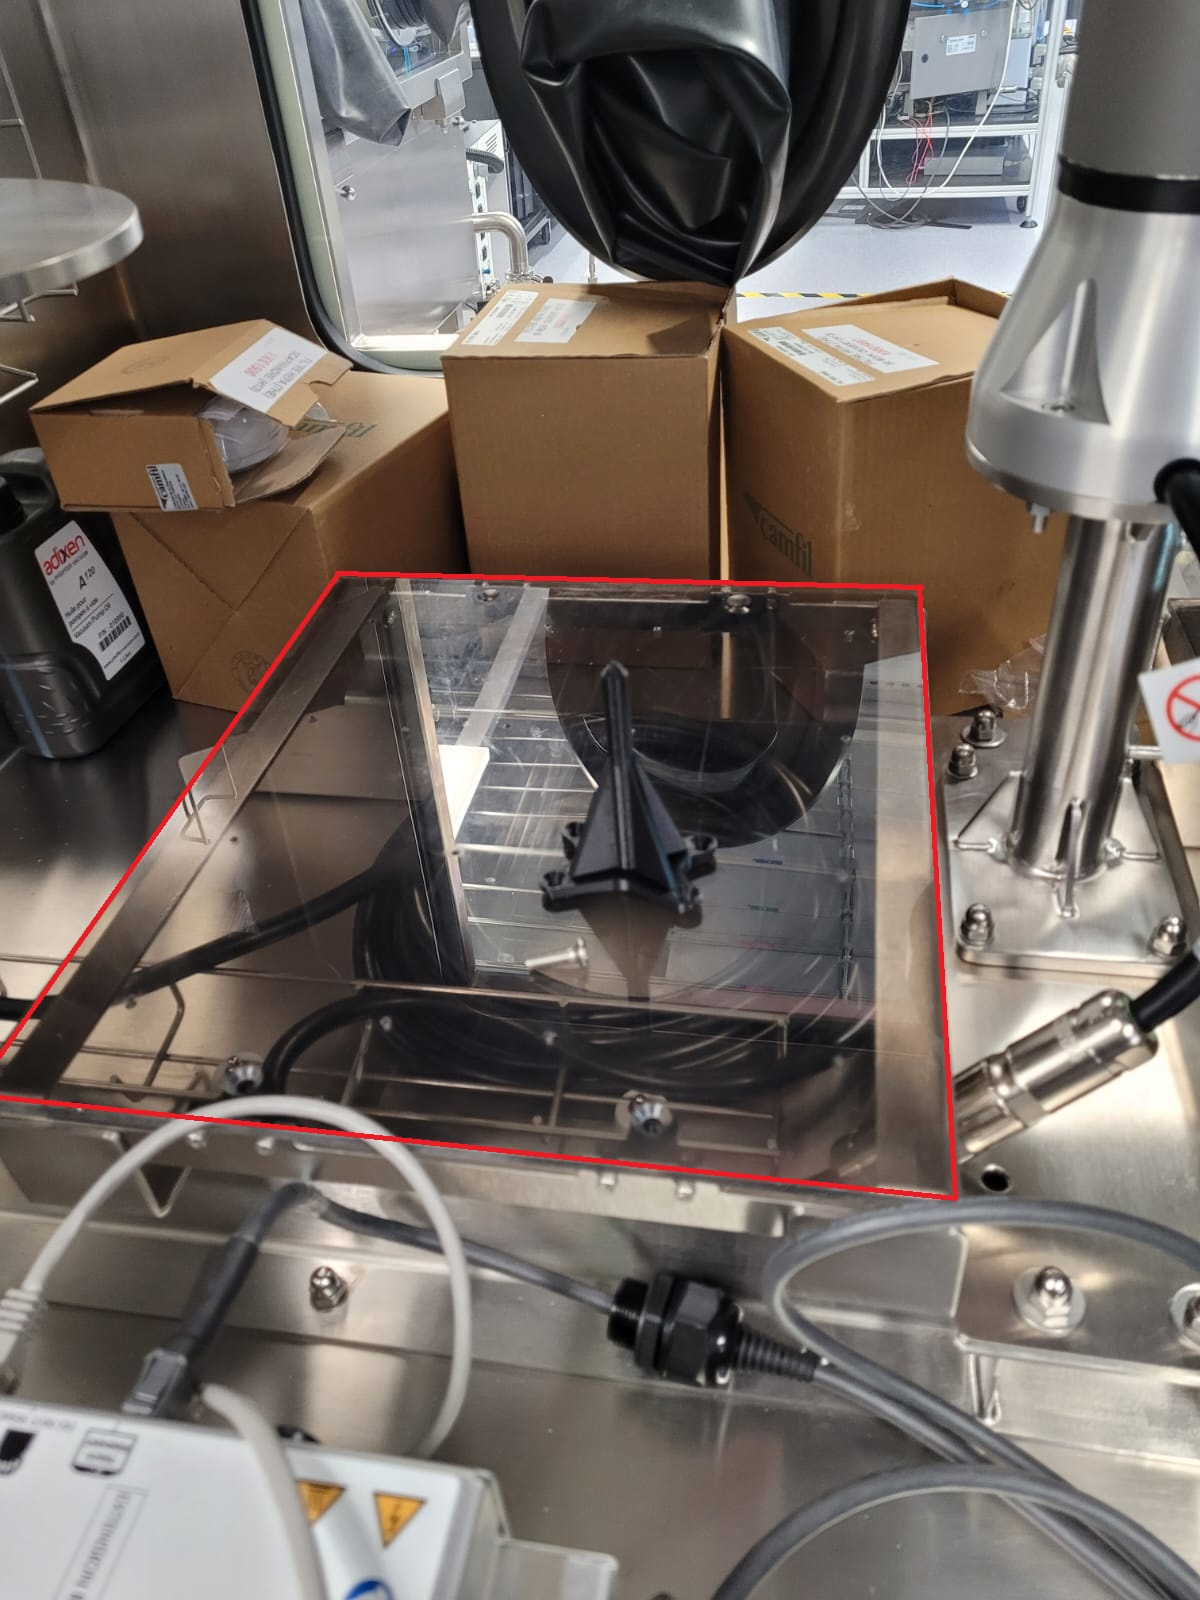
\includegraphics[width=\textwidth/2]{assets/figures/Hardware/plan/planPickAndPlace.jpeg}
    \caption{Position physique du plan \og{}repPickAndPlace\fg{}}
    \label{img:plan_pickandplace}
\end{figure}
\subsection{Communication avec le robot}\label{subsection:CommunicationRobot}
L'interface \textit{Real-Time Data Exchange} (RTDE) permet l'échange bidirectionnel en temps réel des données entre le robot et le système externe, facilitant ainsi le démarrage des programmes robot et la lecture/écriture des registres nécessaires.

\section{Interaction entre le logiciel et le matériel pour la recombinaison}

\chapter{Hardware}
\section{Défis techniques du Hardware}
Le hardware doit pouvoir manipuler des plaques de microcapsules ou de réacteurs, ainsi que des microcapsules en verre de $\qty{3}{\mm}$ de diamètre en garantissant leur intégrité. Le tout doit être dans un espace confiné.
\section{Recherches de solution}
Pour la recherche des solutions, le hardware a été décomposé par les fonctions suivantes : 
\begin{itemize}
    \item saisie et dépose des microcapsules;
    \item déplacement des microcapsules;
    \item saisie et dépose des plaques.
\end{itemize} 
La position des plaques dans la glove box a également été étudié avec $6$ configurations différentes.
\subsection{Saisie et dépose des microcapsules}
Pour la saisie des microcapsules, les grandes familles de solutions proposées sont : 
\begin{itemize}
    \item Aspiration;
    \item Mécanique; \begin{itemize}
        \item Pince à doigt;
        \item Pince Gecko.
    \end{itemize}
\end{itemize}
\subsubsection*{Avantage et inconvénients}
\begin{table}[H]
    \caption{Avantages et inconvénients des solutions de saisie des microcapsules}
    \begin{tabular}{@{}cll@{}}
    \toprule
    Solution      & \multicolumn{1}{c}{Avantages}                                                                                                   & \multicolumn{1}{c}{Inconvénient}                                                                                                                                  \\ \midrule
    Aspiration    & \begin{tabular}[c]{@{}l@{}}- Exerce moins de pression directe \\ - Simple à installer\\ - Nécessite peu d'entretien\end{tabular} & \begin{tabular}[c]{@{}l@{}}- Apporter l'énergie pneumatique\\ - Bruyant\end{tabular}                                                                     \\
    Pince à doigt & \begin{tabular}[c]{@{}l@{}}- Contrôle précis\\ - Faible coût\end{tabular}                                                        & \begin{tabular}[c]{@{}l@{}}- Maintenance fréquente\\ - Ne convient pas au petits objets\\ - Espace limité, pour pouvoir ouvrir \\ et fermer la pince \\ - Nécessite un contrôle de force\end{tabular} \\
    Pince Gecko   & \begin{tabular}[c]{@{}l@{}}- Saisie non intrusive\\ - Ne nécessite pas de source \\ d'énergie externe\end{tabular}                            & \begin{tabular}[c]{@{}l@{}}- Capacité de charge\\ - Nécessite un nettoyage pour maintenir \\  l'adhérence\\ - Détachement complexe\end{tabular}     \\ \bottomrule
    \end{tabular}
\end{table}
\subsection{Déplacement des microcapsules}
Pour le déplacement des \glspl{microcapsule} de leur plaque jusqu'aux réacteurs, trois idées ont été étudiées : 
\begin{itemize}
    \item Transport pneumatique par tube;
    \item convoyeur;
    \item robot.
\end{itemize}
\subsection*{Transport pneumatique par tube}
Le système de transport pneumatique par tube, serait des tuyaux dans lesquelles naviguent les \glspl{microcapsule} grâce à une différence de pression de chaque côté de la \gls{microcapsule}. Ce système est déjà présent dans les hôpitaux et dans les grandes surfaces.
\begin{figure}[h!]
    \centering
    \begin{subfigure}{0.45\textwidth}
        \centering
        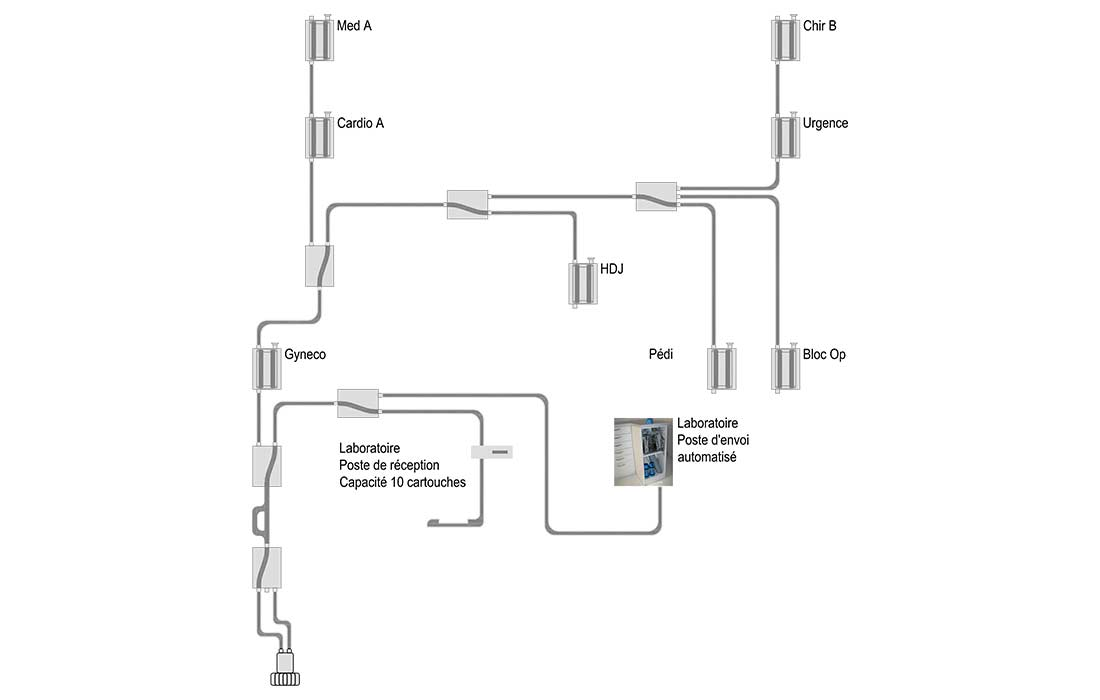
\includegraphics[width=\linewidth]{assets/figures/Hardware/transport_pneu/reseau_pneumatique_hopital.jpg}
        \caption{Schéma d'un réseau de transport pneumatique\footnotemark}
    \end{subfigure}\hfill
    \begin{subfigure}{0.45\textwidth}
        \centering
        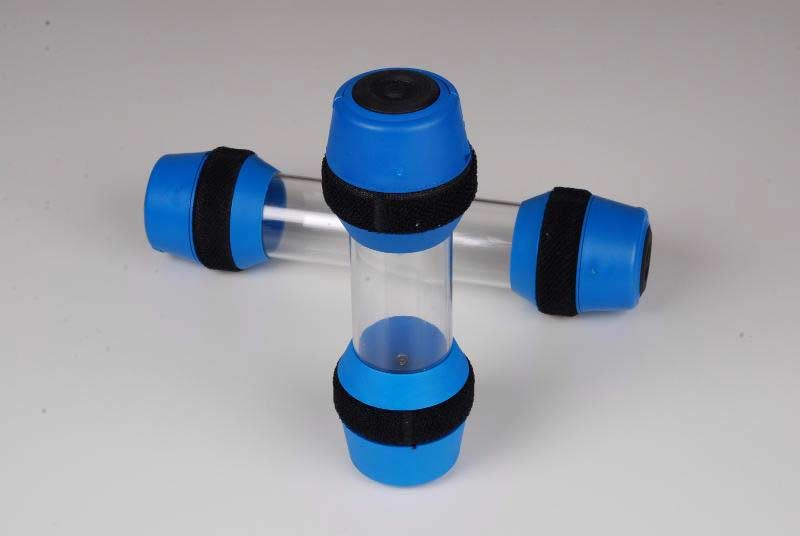
\includegraphics[width=\linewidth]{assets/figures/Hardware/transport_pneu/cartouche_transport_pneu.jpg}
        \caption{Cartouche de transport\footnotemark}
    \end{subfigure}
    \caption{Exemples de réseau de transport pneumatique par tube}
\end{figure}
\footnotetext[1]{\href{https://www.transport-pneumatique.fr/transport-pneumatique-centres-hospitaliers/}{https://www.transport-pneumatique.fr/transport-pneumatique-centres-hospitaliers/}}
\footnotetext[2]{\href{https://www.transport-pneumatique.fr/cartouches-pochettes/}{https://www.transport-pneumatique.fr/cartouches-pochettes/}}
\subsection*{Transport par convoyeur}
Pour déplacer les \glspl{microcapsule}, un convoyeur peut être utilisé, il faut néanmoins que le convoyeur soit adapté au \gls{microcapsule}, les \glspl{microcapsule} étant cyclindriques, elles risquerait de rouler sur un convoyeur à bande lisse, mais une bande à tasseau (\cf \autoref{img:convoyeur_bande_tasseau}) ou un demi-tube  (\cf \autoref{img:convoyeur_tube}) conviendraient parfaitement.
\begin{figure}[h!]
    \centering
    \begin{subfigure}{0.45\textwidth}
        \centering
        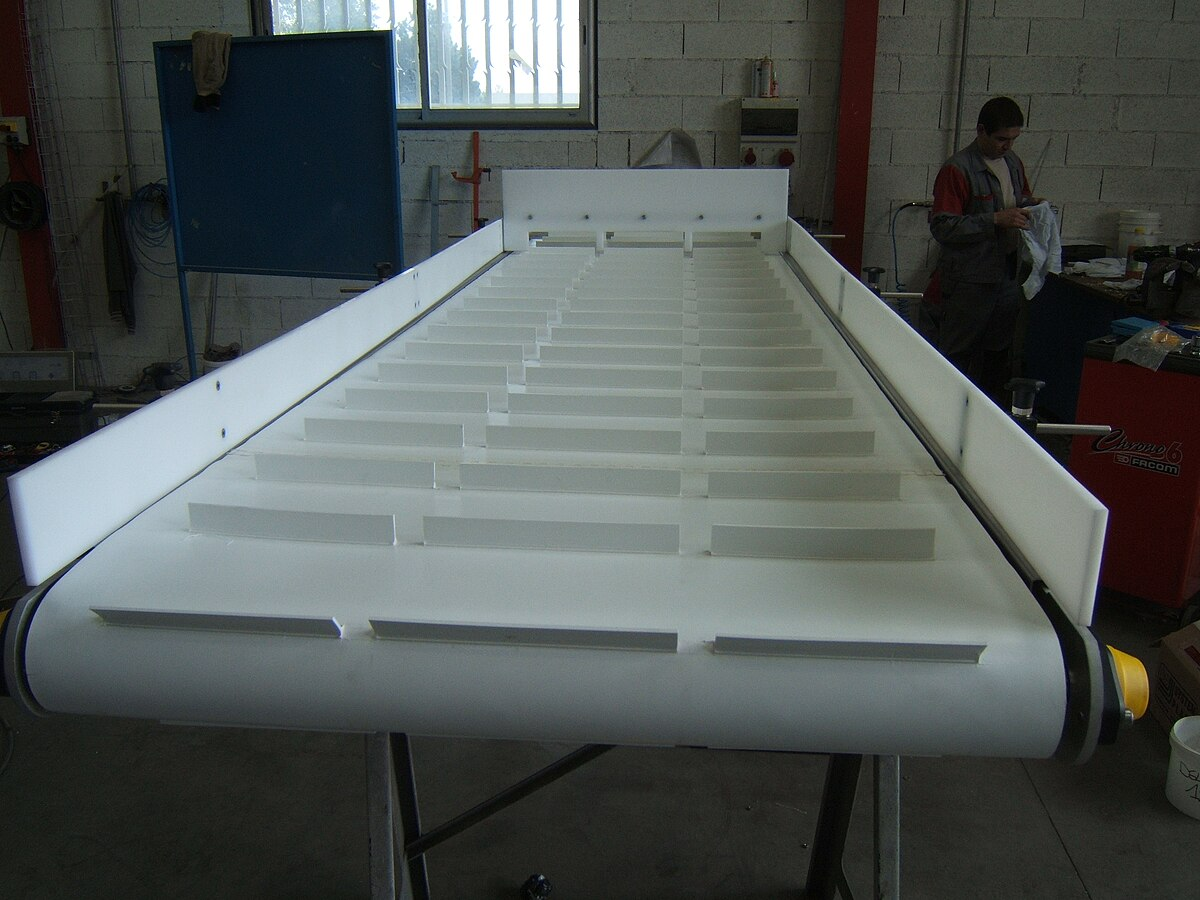
\includegraphics[width=\linewidth]{assets/figures/Hardware/transport_conv/convoyeur_tasseau.JPG}
        \caption{Convoyeur avec bande à tasseaux\footnotemark}
        \label{img:convoyeur_bande_tasseau}
    \end{subfigure}\hfill
    \begin{subfigure}{0.45\textwidth}
        \centering
        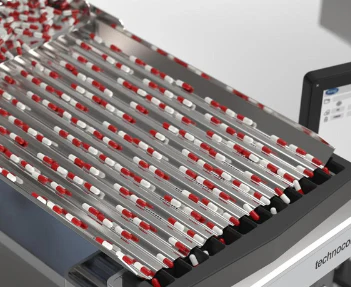
\includegraphics[width=\linewidth]{assets/figures/Hardware/transport_conv/convoyeur_tube.png}
        \caption{Convoyeur à tube\footnotemark}
        \label{img:convoyeur_tube}
    \end{subfigure}
    \caption{Exemple de convoyeur}
\end{figure}
\footnotetext[2]{\href{https://fr.m.wikipedia.org/wiki/Convoyeur}{https://fr.m.wikipedia.org/wiki/Convoyeur}}
\footnotetext[3]{\href{https://doser-compter.com/products/ligne-de-comptage-king}{https://doser-compter.com/products/ligne-de-comptage-king}}
Quant aux différents moyens de mouvoir les \glspl{microcapsule}, il y a : 
\begin{itemize}
    \item les vibrations;
    \item le déplacement de la bande;
    \item la gravité.
\end{itemize}

La dernière option nécessite des surface lisses, que le système soit en pente et le temps de déplacement n'est pas réglable. Les deux autres solutions ne se distinguent pas vraiment pour l'instant, car dans tous les cas, l'utilisation d'un moteur électrique est nécessaire.

\subsection*{Déplacement à l'aide d'un robot}
Pour le déplacement des \glspl{microcapsule}, seuls les axes $T_x, T_y~\text{et}~T_z$ sont nécessaires, soit $3$ degrés de liberté. Un robot de type \textit{SCARA}, cylindrique ou Delta peuvent correspondre.

\subsection*{Avantages et inconvénients}
\begin{table}[H]
    \caption{Anvantages et inconvénients des solution de transport des \glspl{microcapsule}}
    \begin{tabular}{@{}cll@{}}
    \toprule
    Solution      & \multicolumn{1}{c}{Avatanges}                                                                                                   & \multicolumn{1}{c}{Inconvénient}                                                                                                                                  \\ \midrule
    Transport pneumatique par tube    & \begin{tabular}[c]{@{}l@{}}\end{tabular} & \begin{tabular}[c]{@{}l@{}}- Peu modulable\\ - Bruyant\\ - Aiguillage complexe\end{tabular}                                                                     \\
    Convoyeur & \begin{tabular}[c]{@{}l@{}}- \\ - \end{tabular} & \begin{tabular}[c]{@{}l@{}}- Maintenance fréquente\\ - Ne convient pas au petits objets\\ - Espace limité, pour pouvoir ouvrir \\ et fermer la pince \\ - Nécessite un contrôle de force\end{tabular} \\
    Robot   & \begin{tabular}[c]{@{}l@{}}- Place\\ - Modulable \\ \end{tabular}                            & \begin{tabular}[c]{@{}l@{}}- Coût\\ - Nécessite un nettoyage pour conserver \\  l'adhérence dans le temps\\ - Détachement complexe\end{tabular}     \\ \bottomrule
    \end{tabular}
\end{table}

\subsection{Analyse des solutions}
De par la complexité et le manque de modularité du transport pneumatique et du convoyeur, le choix d'utiliser un robot a été choisi.

La position des plaques dans la \textit{glove box} est importante pour la suite, elle permettra de choisir le type de robot à utiliser.
Il est important de savoir comment placer les deux plaques dans la \textit{glove box}.
\subsubsection{Positionnement des plaques dans la \textit{glove box}}
Pour la position des plaques, les solutions trouvées sont : 
\begin{enumerate}
    \item Les plaques ne bougent pas et restent dans les sas;
    \item Les plaques sont positionées symétriquement par rapport au centre de la \textit{glove box};
    \item La plaque de microcapsules est déplacée à côté de la plaque de réacteur, cette dernière ne bouge pas;
    \item La plaque de microcapsules reste dans le sas tandis que la plaque de réacteur est transportée à ses côtés;
    \item Les deux plaques sont mises l'une à côté de l'autre en étant plus proches du stock;
    \item Les deux plaques sont mises l'une à côté de l'autre en étant plus proches de la sortie;
\end{enumerate}
Le temps de cycle est le suivant :
\begin{align*}
    tpsCycle &= tpsDeplacementPlaquesCapsule + tpsDeplacement_{Capsule} \\
    &+ tpsAttentePlaque + tpsDeplacement_{PlaquesReacteur}\\
    &= nbrePlaques\cdot \frac{d_{PlaqueMicrocapsules}}{v_{robot}} \\&+ nbreMicrocapsules\cdot \frac{d_{EntrePlaque}}{v_{robot}} \\
    &+ 2\cdot nbrePlaques\cdot tpsAttente + \frac{d_{PlaqueReacteur}}{v_{robot}}
\end{align*}

Certaines valeurs ne peuvent être connue que lors de la mise en route, notamment l'accélération, la vitesse d'approche, il est nécessaire de faire certaines hypothèses. Les distances sont également arbitraires afin de se faire une idée du temps de cycle des solutions. Ici, la position optimale n'est pas recherché.
En utilisant les hypothèses suivantes :
\begin{itemize}
    \item $v_{robot} = \qty{1}{\frac{\m}{\s}}$;
    \item $d_{EntrePlaque} = \qtylist[list-units = single]{1.33; 0.3; 0.3; 0.3; 0.3; 0.3}{\m\per\s}$;
    \item $d_{PlaqueMicrocapsules} = \qtylist[list-units = single]{0; 0.515; 1.03; 0; 0.83; 0.2 }{\m}$;
    \item $d_{PlaqueReacteur} =      \qtylist[list-units = single]{0; 0.515; 0; 1.03; 0.2; 0.83 }{\m}$;
    \item $d_{PlaqueMicrocapsules} = \qtylist[list-units = single]{0; 0.515; 1.03; 0; 0.83; 0.2 }{\m}$;
    \item L'accélération du robot est infinie;
    \item La vitesse d'approche n'est pas prise en compte.
\end{itemize}
Avec ces informations, il est possible de calculer le temps moyen d'un cycle (\cf \autoref{img:graph_temps_cycle_moyen_sequentielle}) en fonction du nombre de microcapsule demandées ainsi que du nombre de microcapsule par plaque, et ce, pour chaque solution.
\begin{figure}[H]
    \centering
    \includesvg[width = \textwidth]{assets/figures/Hardware/recherchSoluce/temps_cycle_moyen_toute_solution.svg}
    \caption{Temps de cycle moyen des différentes solutions}
    \label{img:graph_temps_cycle_moyen_sequentielle}
\end{figure}
Il est possible de voir que les solutions $4$ et $6$ semblent les plus rapide. Le temps d'attente des plaques est cependant très important, environ $84~\%$ du temps total. Pour réduire ce délai, il peut être intéressant de paralléliser les tâches.
\subsubsection{parallélisation des robots}
La parallélisation des tâches consiste à effectuer le \textit{pick and place} des microcapsules, la prise et la dépose des plaques indépendamment.
De par la configuration des sas, il n'est possible d'y mettre qu'une seule plaque, la parallélisation des solutions $\numlist{1; 3; 4}$ n'est donc pas possible.

\begin{figure}[H]
    \centering
    \includesvg[width = \textwidth]{assets/figures/Hardware/recherchSoluce/para.svg}
    \caption{Comparaison du temps de cycle des solutions en fonction du nombre de microcapsules par plaque}
    \label{img:graph_temps_cycle_para}
\end{figure}

Sur \autoref{img:graph_temps_cycle_para}, il est possible de voir que les solutions parallélisées ont toujours un temps de cycle inférieur aux solutions séquentielles tant que le nombre de microcapsules par plaque est inférieur au nombre de microcapsules demandées.
Plus le nombre de microcapsule demandées est élevé, plus le gain de temps est significatif, allant, en moyenne, de $1.3~\%$ pour $48$ microcapsules à $27~\%$ pour $240$ microcapsules.
\section{Présentation de la solution choisie}
L'utilisation d'un seul robot positionné au centre de la \textit{glove box}, qui s'occupera de déplacer les plaques ainsi que de faire le \textit{pick and place} des microcapsules a été retenue.
Cette décision est due à : 
\begin{itemize}
    \item un robot déjà présent dans le laboratoire;
    \item la grande flexibilité de cette solution (la \textit{glove box} sera utilisée pour d'autres processus par la suite).
\end{itemize}
\section{Description du matériel utilisé}
Voici la liste de matériel utilisé lors du TB : 
\begin{itemize}
    \item Robot \og{}UR3e\fg{};
    \item Pince \og{}Hand-E\fg{};
    \item Adaptation de la pince précédente sur mesure;
    \item Module d'aspiration;
    \item Support pour les plaques.
\end{itemize}
\section{Intégration}
Afin de maximiser l'espace accessible par le robot, ce dernier a été surélevé (\cf \autoref{img:integration_robot_glove}). La moitié gauche est réservée pour le \textit{pick and place} des microcapsules, tandis que la partie à droite servira pour la suite du processus.
Pour les outils, la pince se met sur la bride du robot et elle possède deux trous taraudés qui seront utilisé pour fixer le module d'aspiration (\cf \autoref{img:integration_pince}).
L'outil pour saisir les plaques fait un angle à $\qty{45}{\degree}$ pour pouvoir déposer les plaques sur tout le plan \textit{repPickAndPlace}. Afin de gagner de la place, les deux outils sont placés dans des directions opposées.
\begin{figure}[ht]
    \centering
    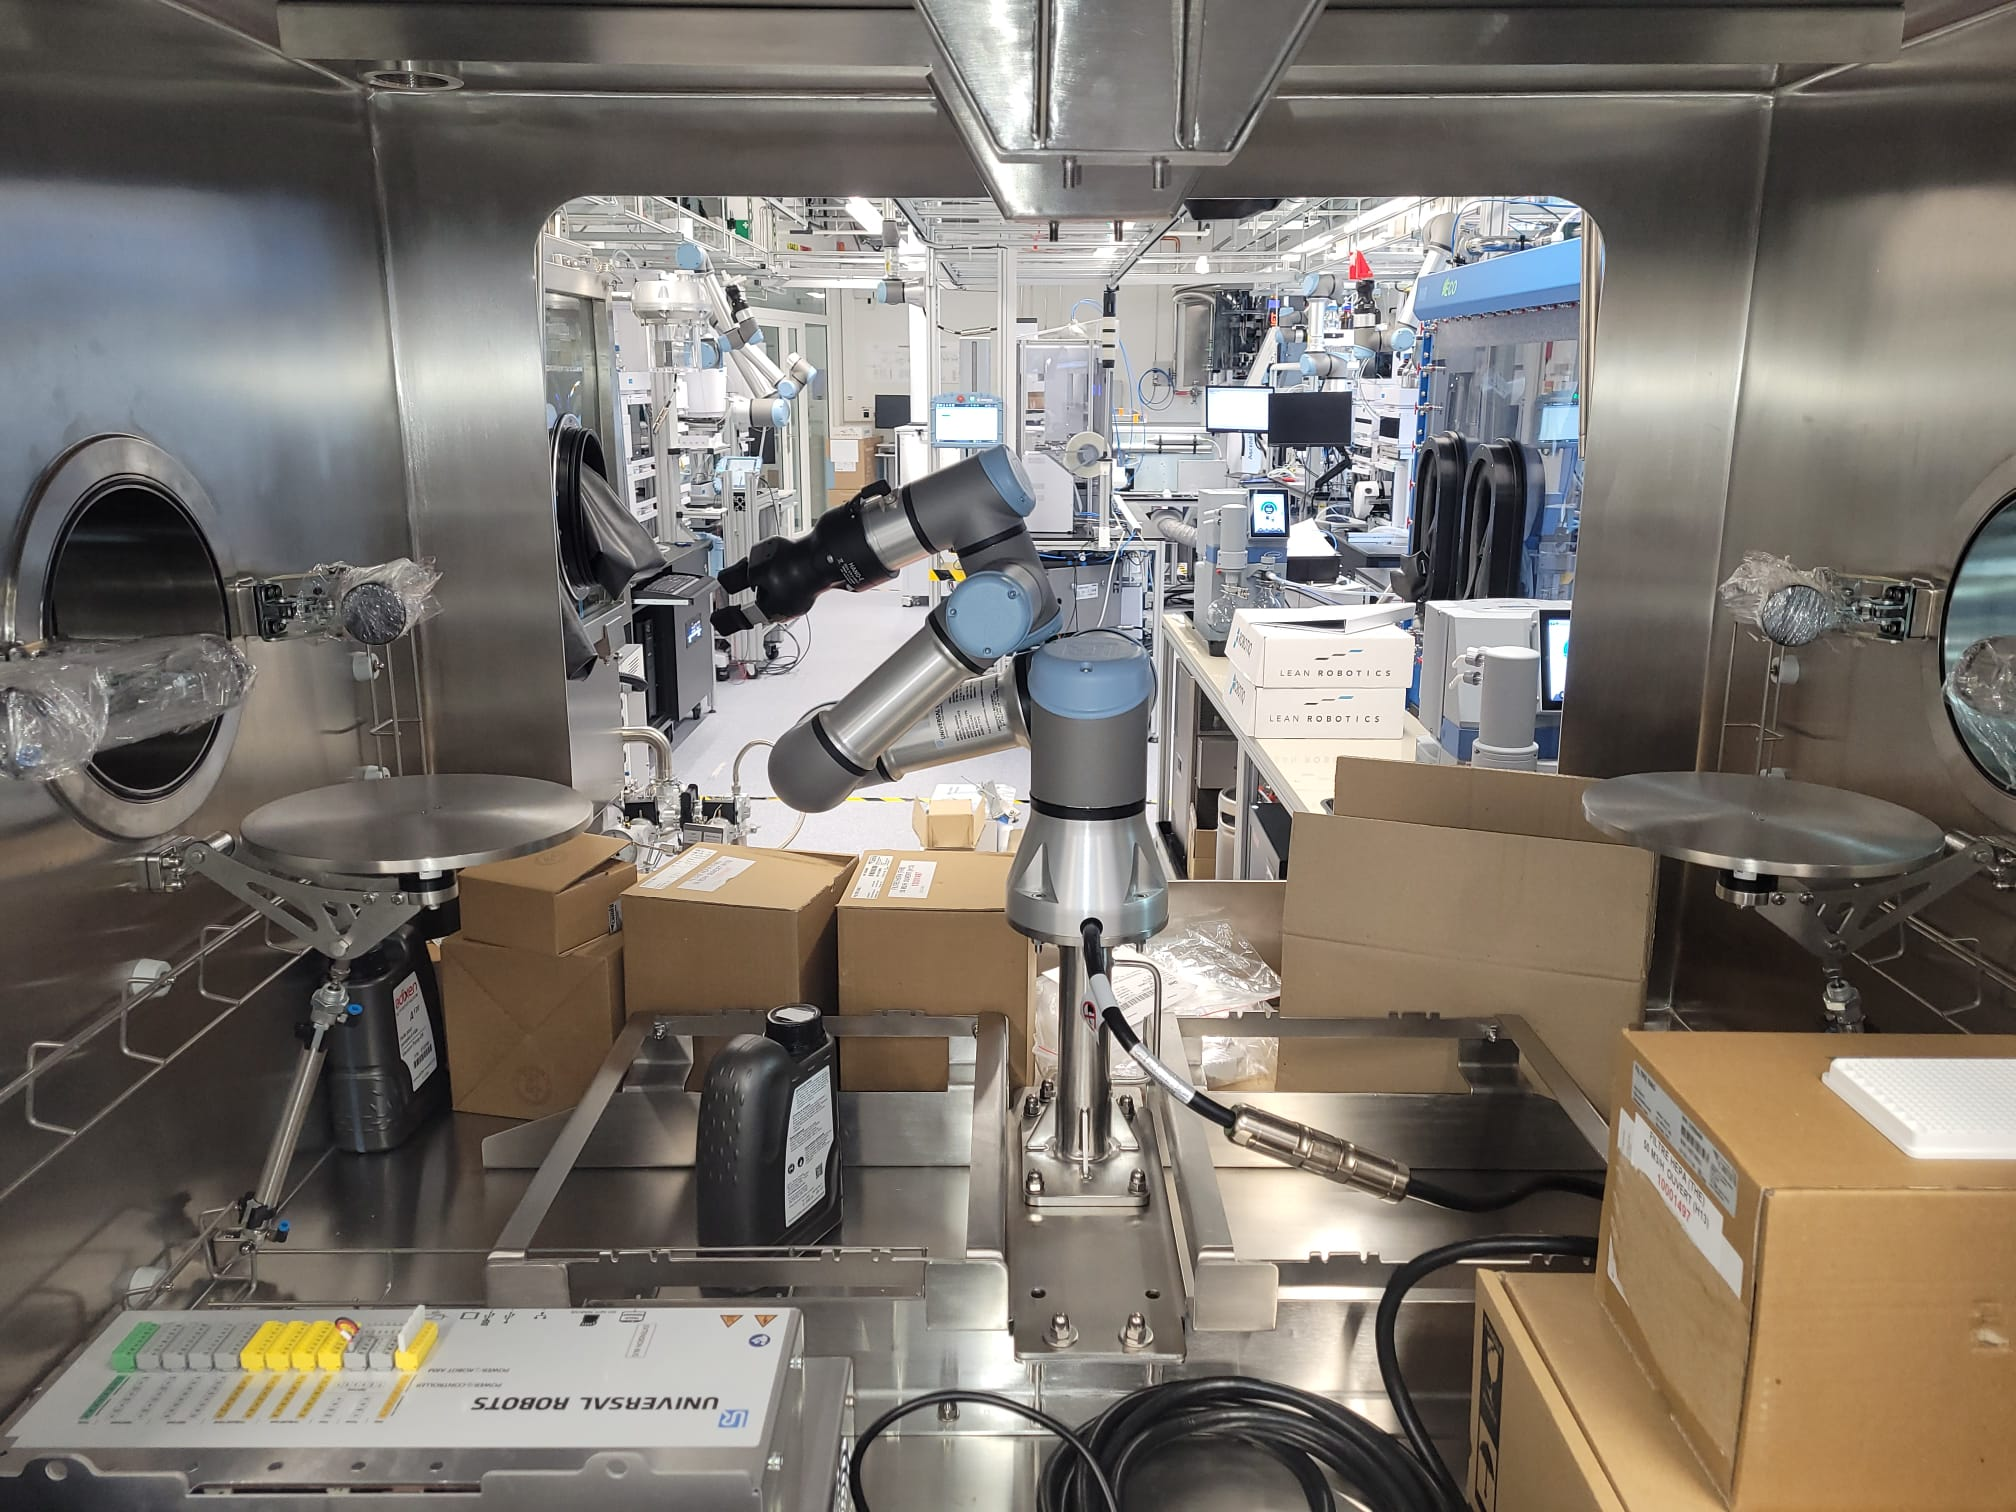
\includegraphics[width = 0.5\textwidth]{assets/figures/Hardware/gloveBox.jpeg}
    \caption{Intégration du robot dans la \textit{glove box}}
    \label{img:integration_robot_glove}
\end{figure}
\begin{figure}[ht]
    \centering
    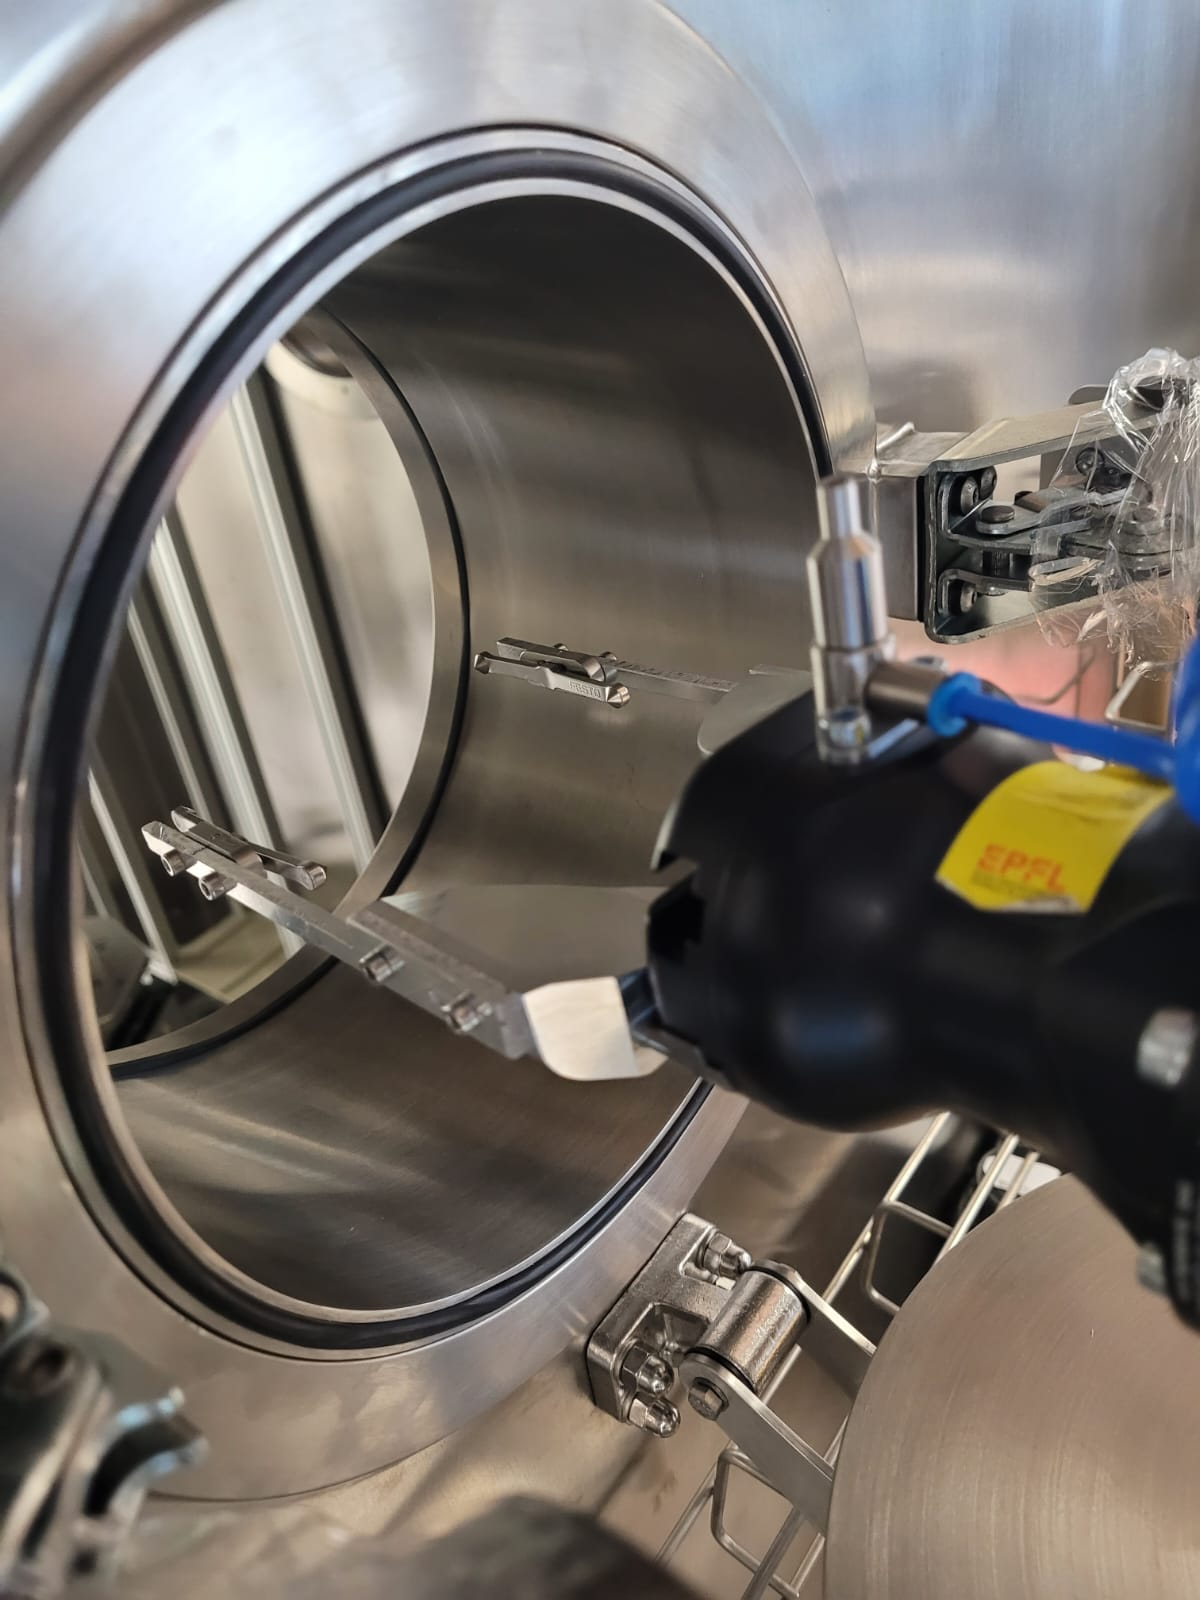
\includegraphics[width = 0.5\textwidth]{assets/figures/Hardware/outil_complet.jpeg}
    \caption{Module d'aspiration}
    \label{img:integration_pince}
\end{figure}

\chapter{Implémentation et intégration Hardware-Software}
\section{Développement du logiciel}
\section{Intégration avec le Hardware}
\section{Tests de validation et calibrage du matériel}

\chapter{Résultat et Analyse}
\section{Performance du système}
\section{Analyse des erreurs}

\chapter{Discussion}

\chapter{Conclusion}
Ce projet de Bachelor a permis de dévelloper un système robotisé innovant pour la recombinaison des \glspl{microcapsule} chimiques dans un laboratoire de recherche. Les contributions principales incluent la conception et l'integration d'un robot dans une \gls{glovebox}, et la création d'un algorithme d'optimisation permettant de maximiser le nombre de recette réalisable.

L'ensemble du système répond aux éxigences initiales initiales en matières de précision, de fiabilité et de sécurité, tout en offrant une grande flexibilité pour des applications futures.Les résultats obtenus démontrent que l'automatisation de la recombinaison peut considérablement accélérer le processus expérimental, réduisant les erreurs humaines et augmentant l'efficacité global.

Cependant certains points, comme le réseau pneumatique, n'ont pas pu être réalisée à cause d'un manque de temps.

Des axes d'amélioration existent. Le temps de calcul de l'algorithme, la robustesse des outils et la gestion des risques liés à la manipulation sont des aspects à améliorer. L'ajout d'un module d'intelligence artificielle et l'amélioration des outils physique pourrait augmenter le rendement de la recombinaison.

En conclusion, ce travail de représente une avancée vers l'automatisation complète des tâches dans le laboratoire.

\vfil
\hspace{8cm}\makeatletter\@author\makeatother\par
\hspace{8cm}\begin{minipage}{5cm}
\end{minipage}


\clearpage
\printbibliography

\appendix
\appendixpage
\addappheadtotoc



\let\cleardoublepage\clearpage
\backmatter

\label{glossaire}
\printnoidxglossary
\label{index}
\printindex

% Le colophon est le dernier élément d'un document qui contient des notes de l'auteur concernant la mise en page et l'édition du document : il est parfaitement optionnel.
\input{colophon.tex}

\end{document}
